\section{Results}
\label{sec:result}

We run a Metropolis-Hastings algorithm for 2,000,000 iterations. To reduce autocorrelation between iterations, we thin the sample and only keep the sampled values every 100 steps, resulting in a final posterior sample of 20,000.

\subsection{Results on Firms' Preferences}

\Cref{fig:traceplot_alpha} show the trace plots of $\alpha$, firms' preference parameters for countries' log GDP, log GDP per capita, democracy, and labor quality. The plots show that the MCMC chains do converge after the 5000\textsuperscript{th} iterations with the exception of the preference parameter for log GDP per capita. Our interpretation of this parameter is therefore more speculative.

\begin{figure}[!ht]
\centering
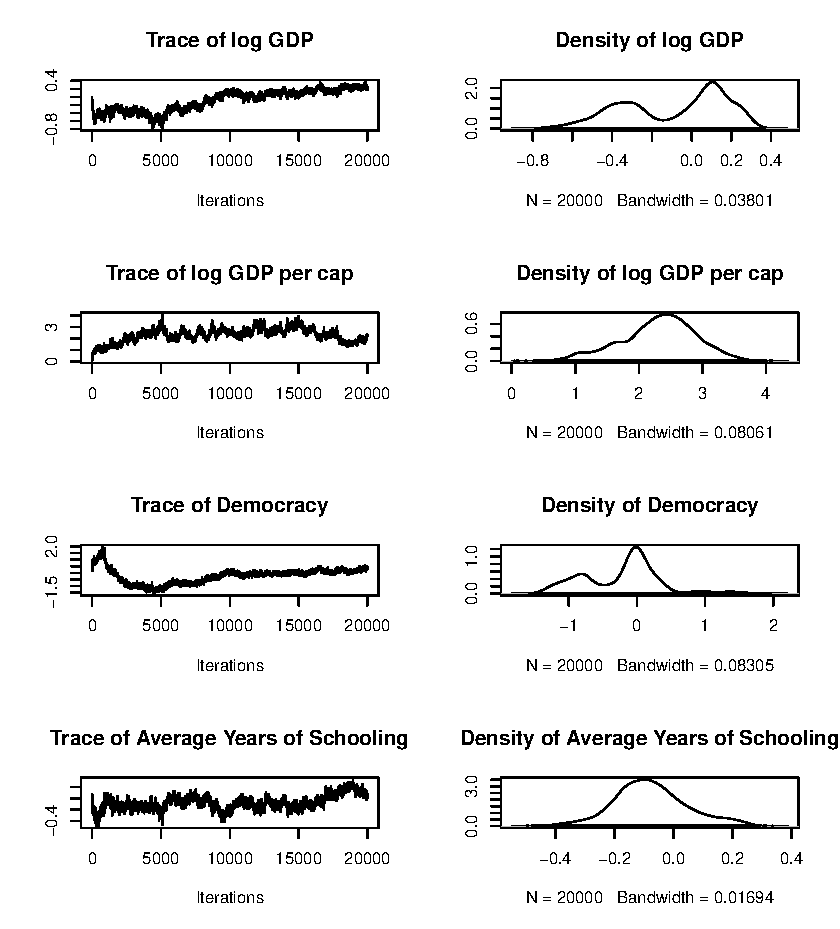
\includegraphics[width=\textwidth,keepaspectratio]{../figure/traceplot_alpha}
\caption{Traceplot.}
\label{fig:traceplot_alpha}
\end{figure}

The estimated parameters can be interpreted naturally in the utility space as the relative weights that firms assign to countries' characteristics.\footnote{In the utility space, the scale of the parameters do not matter. Consider two scenarios: 1) country A offers 10 ``utilities'' while country B offers 50; 2) country A offers 1 ``utility'' while country B offers 5. These two scenarios are identical since the firm will choose country B over country A.} For example, since the value of firms' preference for democracy is -0.305 and for log GDP is 0.734, it means that being an autocracy is worth 0.305 / 0.734 of 1 unit increase in log GDP. Interpreting on the GDP scale, it means that being an autocracy is worth 0.305 / 0.00734 = 41.5 times a 1\% increase in GDP. For our sample of 

One surprising result is the 




Skill does not matter, host GDP is negative, host gdppc is positive \citep{Eicher2012}

Host GDP is negative, host GDP per capita is positive, host democracy is positive, agree with 
